\documentclass[a4paper,man,hidelinks,floatsintext]{apa7}
% This LaTeX output is designed to use APA7 style and to run on local TexLive-installation (use pdflatex) as well as on web interfaces (e.g., overleaf.com).
% To use APA6 style change apa7 to apa6 in the first line (\documentclass), comment or remove the \addORCIDlink line, and change the order of \caption and \label lines for the figures.
% If you prefer postponing your figures and table until after the reference list, instead of having them within the body of the text, please remove the ",floatsintext" from the documentclass options.
% Further information on these styles can be found here: https://www.ctan.org/pkg/apa7 and here: https://www.ctan.org/pkg/apa6

\usepackage[british]{babel}
\usepackage[utf8]{inputenc}
\usepackage{amsmath}
\usepackage{graphicx}
\usepackage[export]{adjustbox}
\usepackage{csquotes}
\usepackage[style=apa,sortcites=true,sorting=nyt,backend=biber]{biblatex}
\DeclareLanguageMapping{british}{british-apa}
\addbibresource{article.bib}

\title{APA-Style Manuscript with jamovi Results}
\shorttitle{jamovi Results}
\author{Full Name}
\leftheader{Last name}
\affiliation{Your Affilitation}
% addORCIDlink is only available from apa7
\authornote{\addORCIDlink{Your Name}{0000-0000-0000-0000}\\
More detailed information about how to contact you.\\
Can continue over several lines.
}

\abstract{Your abstract here.}
\keywords{keyword 1, keyword 2}

\begin{document}
%\maketitle

% Your introduction starts here.

%\section{Methods}
% Feel free to adjust the subsections below.

%\subsection{Participants}
% Your participants description goes here.

%\subsection{Materials}
% Your description of the experimental materials goes here.

%\subsection{Procedure}
% Your description of the experimental procedures goes here.

%\subsection{Statistical Analyses}
%Statistical analyses were performed using jamovi \parencite{jamovi}, and the R statistical language \parencite{R}, as well as the module / package GAMLj \parencite{GAMLj}.

%\section{Results}

% =========================================================================================================


<h1 contenteditable="" spellcheck="false">Results</h1>
           
      
        <p></p>
      
    
      
      
    
            <h1 contenteditable="" spellcheck="false">Mixed Model</h1>
           
      
        <p></p>
      
    
\begin{table}[!htbp]
\caption{Model Info}
\label{tab:Table_1}
\begin{adjustbox}{max size={\columnwidth}{\textheight}}
\centering
\begin{tabular}{ll}
\hline
Info                  & ~                                                                                                                               \\
\hline
Estimate              & Linear mixed model fit by REML                                                                                                  \\
Call                  & Rating ~ 1 + Condition + Vowel + Gender + Condition:Vowel + Condition:Gender + Vowel:Gender + Gender:Vowel:Condition+( 1 | ID ) \\
AIC                   & 43325.002                                                                                                                       \\
BIC                   & 43472.936                                                                                                                       \\
LogLikel.             & -21600.354                                                                                                                      \\
R-squared Marginal    & 0.383                                                                                                                           \\
R-squared Conditional & 0.542                                                                                                                           \\
Converged             & yes                                                                                                                             \\
Optimizer             & bobyqa                                                                                                                          \\
\hline
\end{tabular}
\end{adjustbox}
\begin{tablenotes}[para,flushleft] {
\small
}
\end{tablenotes}
\end{table}
      
        <p></p>
      
    <h2>Model Results</h2>
      
        <p></p>
      
    
\begin{table}[!htbp]
\caption{Fixed Effect Omnibus tests}
\label{tab:Table_2}
\begin{adjustbox}{max size={\columnwidth}{\textheight}}
\centering
\begin{tabular}{lrrrr}
\hline
~                                            &      F & Num df & Den df &               p \\
\hline
Condition                                    & 967.24 &      4 &   4888 & \textless~0.001 \\
Vowel                                        &   4.64 &      2 &   4888 &           0.010 \\
Gender                                       &  14.40 &      1 &   4888 & \textless~0.001 \\
Condition ~$\times$~ Vowel                   &   3.51 &      8 &   4888 & \textless~0.001 \\
Condition ~$\times$~ Gender                  &  33.72 &      4 &   4888 & \textless~0.001 \\
Vowel ~$\times$~ Gender                      &  13.99 &      2 &   4888 & \textless~0.001 \\
Condition ~$\times$~ Vowel ~$\times$~ Gender &   6.88 &      8 &   4888 & \textless~0.001 \\
\hline
\end{tabular}
\end{adjustbox}
\begin{tablenotes}[para,flushleft] {
\small
\textit{Note.}~Satterthwaite method for degrees of freedom. \\
}
\end{tablenotes}
\end{table}
      
        <p></p>
      
    
\begin{table}[!htbp]
\caption{Fixed Effects Parameter Estimates}
\label{tab:Table_3}
\begin{adjustbox}{max size={\columnwidth}{\textheight}}
\centering
\begin{tabular}{llrrrrr}
\hline
Names                                           & Effect                                                                      & Estimate &    SE &     df &       t &               p \\
\hline
(Intercept)                                     & (Intercept)                                                                 &   59.531 & 1.959 &   32.0 &  30.396 & \textless~0.001 \\
Condition1                                      & harmonic - reference                                                        &  -15.759 & 0.851 & 4888.0 & -18.523 & \textless~0.001 \\
Condition2                                      & estimated - reference                                                       &  -36.639 & 0.851 & 4888.0 & -43.066 & \textless~0.001 \\
Condition3                                      & synthesized - reference                                                     &  -41.607 & 0.851 & 4888.0 & -48.905 & \textless~0.001 \\
Condition4                                      & anchor - reference                                                          &  -42.458 & 0.851 & 4888.0 & -49.905 & \textless~0.001 \\
Vowel1                                          & i - ( a, i, o )                                                             &    0.578 & 0.380 & 4888.0 &   1.520 &           0.129 \\
Vowel2                                          & o - ( a, i, o )                                                             &   -1.159 & 0.380 & 4888.0 &  -3.047 &           0.002 \\
Gender1                                         & male - female                                                               &   -2.040 & 0.538 & 4888.0 &  -3.791 & \textless~0.001 \\
Condition1 ~$\times$~ Vowel1                    & harmonic - reference ~$\times$~ i - ( a, i, o )                             &    0.995 & 1.203 & 4888.0 &   0.827 &           0.408 \\
Condition2 ~$\times$~ Vowel1                    & estimated - reference ~$\times$~ i - ( a, i, o )                            &    1.497 & 1.203 & 4888.0 &   1.244 &           0.213 \\
Condition3 ~$\times$~ Vowel1                    & synthesized - reference ~$\times$~ i - ( a, i, o )                          &    3.228 & 1.203 & 4888.0 &   2.683 &           0.007 \\
Condition4 ~$\times$~ Vowel1                    & anchor - reference ~$\times$~ i - ( a, i, o )                               &   -2.121 & 1.203 & 4888.0 &  -1.763 &           0.078 \\
Condition1 ~$\times$~ Vowel2                    & harmonic - reference ~$\times$~ o - ( a, i, o )                             &   -1.963 & 1.203 & 4888.0 &  -1.631 &           0.103 \\
Condition2 ~$\times$~ Vowel2                    & estimated - reference ~$\times$~ o - ( a, i, o )                            &   -2.818 & 1.203 & 4888.0 &  -2.342 &           0.019 \\
Condition3 ~$\times$~ Vowel2                    & synthesized - reference ~$\times$~ o - ( a, i, o )                          &   -2.978 & 1.203 & 4888.0 &  -2.475 &           0.013 \\
Condition4 ~$\times$~ Vowel2                    & anchor - reference ~$\times$~ o - ( a, i, o )                               &    1.094 & 1.203 & 4888.0 &   0.909 &           0.363 \\
Condition1 ~$\times$~ Gender1                   & harmonic - reference ~$\times$~ male - female                               &    3.840 & 1.702 & 4888.0 &   2.257 &           0.024 \\
Condition2 ~$\times$~ Gender1                   & estimated - reference ~$\times$~ male - female                              &   -6.762 & 1.702 & 4888.0 &  -3.974 & \textless~0.001 \\
Condition3 ~$\times$~ Gender1                   & synthesized - reference ~$\times$~ male - female                            &   -7.731 & 1.702 & 4888.0 &  -4.544 & \textless~0.001 \\
Condition4 ~$\times$~ Gender1                   & anchor - reference ~$\times$~ male - female                                 &    8.705 & 1.702 & 4888.0 &   5.116 & \textless~0.001 \\
Vowel1 ~$\times$~ Gender1                       & i - ( a, i, o ) ~$\times$~ male - female                                    &   -1.710 & 0.761 & 4888.0 &  -2.248 &           0.025 \\
Vowel2 ~$\times$~ Gender1                       & o - ( a, i, o ) ~$\times$~ male - female                                    &   -2.301 & 0.761 & 4888.0 &  -3.023 &           0.003 \\
Condition1 ~$\times$~ Vowel1 ~$\times$~ Gender1 & harmonic - reference ~$\times$~ i - ( a, i, o ) ~$\times$~ male - female    &   -6.313 & 2.406 & 4888.0 &  -2.624 &           0.009 \\
Condition2 ~$\times$~ Vowel1 ~$\times$~ Gender1 & estimated - reference ~$\times$~ i - ( a, i, o ) ~$\times$~ male - female   &   -0.408 & 2.406 & 4888.0 &  -0.170 &           0.865 \\
Condition3 ~$\times$~ Vowel1 ~$\times$~ Gender1 & synthesized - reference ~$\times$~ i - ( a, i, o ) ~$\times$~ male - female &    0.974 & 2.406 & 4888.0 &   0.405 &           0.686 \\
Condition4 ~$\times$~ Vowel1 ~$\times$~ Gender1 & anchor - reference ~$\times$~ i - ( a, i, o ) ~$\times$~ male - female      &    4.186 & 2.406 & 4888.0 &   1.740 &           0.082 \\
Condition1 ~$\times$~ Vowel2 ~$\times$~ Gender1 & harmonic - reference ~$\times$~ o - ( a, i, o ) ~$\times$~ male - female    &    2.717 & 2.406 & 4888.0 &   1.129 &           0.259 \\
Condition2 ~$\times$~ Vowel2 ~$\times$~ Gender1 & estimated - reference ~$\times$~ o - ( a, i, o ) ~$\times$~ male - female   &   -6.214 & 2.406 & 4888.0 &  -2.582 &           0.010 \\
Condition3 ~$\times$~ Vowel2 ~$\times$~ Gender1 & synthesized - reference ~$\times$~ o - ( a, i, o ) ~$\times$~ male - female &  -10.020 & 2.406 & 4888.0 &  -4.164 & \textless~0.001 \\
Condition4 ~$\times$~ Vowel2 ~$\times$~ Gender1 & anchor - reference ~$\times$~ o - ( a, i, o ) ~$\times$~ male - female      &   -2.511 & 2.406 & 4888.0 &  -1.044 &           0.297 \\
\hline
\end{tabular}
\end{adjustbox}
\begin{tablenotes}[para,flushleft] {
\small
}
\end{tablenotes}
\end{table}
      
        <p></p>
      
    
\begin{table}[!htbp]
\caption{Random Components}
\label{tab:Table_4}
\begin{adjustbox}{max size={\columnwidth}{\textheight}}
\centering
\begin{tabular}{llrrr}
\hline
Groups   & Name        &   SD & Variance &   ICC \\
\hline
ID       & (Intercept) & 11.1 &      124 & 0.257 \\
Residual & ~           & 18.9 &      358 &     ~ \\
\hline
\end{tabular}
\end{adjustbox}
\begin{tablenotes}[para,flushleft] {
\small
\textit{Note.}~Number of Obs: 4950 , groups: ID 33. \\
}
\end{tablenotes}
\end{table}
      
        <p></p>
      
    
\begin{table}[!htbp]
\caption{Random Effect LRT}
\label{tab:Table_5}
\begin{adjustbox}{max size={\columnwidth}{\textheight}}
\centering
\begin{tabular}{lrrrrr}
\hline
Test     & N. par &   AIC &  LRT &   df &               p \\
\hline
(1 | ID) &   31.0 & 44569 & 1306 & 1.00 & \textless~0.001 \\
\hline
\end{tabular}
\end{adjustbox}
\begin{tablenotes}[para,flushleft] {
\small
}
\end{tablenotes}
\end{table}
      
        <p></p>
      
    
      
      
    
      
        <p></p>
      
    <h2>Post Hoc Tests</h2>
      
        <p></p>
      
    
\begin{table}[!htbp]
\caption{Post Hoc Comparisons - Condition}
\label{tab:Table_6}
\begin{adjustbox}{max size={\columnwidth}{\textheight}}
\centering
\begin{tabular}{lrlrrrrr}
\hline
\multicolumn{3}{c}{Comparison} & \multicolumn{5}{c}{~} \\
\cline{1-3}
Condition   & ~ & Condition   & Difference &    SE &      t &   df & p$_{bonferroni}$ \\
\hline
harmonic    & - & synthesized &     25.848 & 0.851 & 30.382 & 4888 &  \textless~0.001 \\
harmonic    & - & anchor      &     26.699 & 0.851 & 31.382 & 4888 &  \textless~0.001 \\
harmonic    & - & estimated   &     20.881 & 0.851 & 24.543 & 4888 &  \textless~0.001 \\
synthesized & - & anchor      &      0.851 & 0.851 &  1.000 & 4888 &            1.000 \\
reference   & - & harmonic    &     15.759 & 0.851 & 18.523 & 4888 &  \textless~0.001 \\
reference   & - & synthesized &     41.607 & 0.851 & 48.905 & 4888 &  \textless~0.001 \\
reference   & - & anchor      &     42.458 & 0.851 & 49.905 & 4888 &  \textless~0.001 \\
reference   & - & estimated   &     36.639 & 0.851 & 43.066 & 4888 &  \textless~0.001 \\
estimated   & - & synthesized &      4.968 & 0.851 &  5.839 & 4888 &  \textless~0.001 \\
estimated   & - & anchor      &      5.818 & 0.851 &  6.839 & 4888 &  \textless~0.001 \\
\hline
\end{tabular}
\end{adjustbox}
\begin{tablenotes}[para,flushleft] {
\small
}
\end{tablenotes}
\end{table}
      
        <p></p>
      
    
\begin{table}[!htbp]
\caption{Post Hoc Comparisons - Vowel}
\label{tab:Table_7}
\begin{adjustbox}{max size={\columnwidth}{\textheight}}
\centering
\begin{tabular}{lrlrrrrr}
\hline
\multicolumn{3}{c}{Comparison} & \multicolumn{5}{c}{~} \\
\cline{1-3}
Vowel & ~ & Vowel & Difference &    SE &       t &   df & p$_{bonferroni}$ \\
\hline
i     & - & o     &    1.73758 & 0.659 & 2.63667 & 4888 &            0.025 \\
a     & - & i     &    0.00242 & 0.659 & 0.00368 & 4888 &            1.000 \\
a     & - & o     &    1.74000 & 0.659 & 2.64035 & 4888 &            0.025 \\
\hline
\end{tabular}
\end{adjustbox}
\begin{tablenotes}[para,flushleft] {
\small
}
\end{tablenotes}
\end{table}
      
        <p></p>
      
    
\begin{table}[!htbp]
\caption{Post Hoc Comparisons - Gender}
\label{tab:Table_8}
\begin{adjustbox}{max size={\columnwidth}{\textheight}}
\centering
\begin{tabular}{lrlrrrrr}
\hline
\multicolumn{3}{c}{Comparison} & \multicolumn{5}{c}{~} \\
\cline{1-3}
Gender & ~ & Gender & Difference &    SE &    t &   df & p$_{bonferroni}$ \\
\hline
female & - & male   &       2.04 & 0.538 & 3.79 & 4888 &  \textless~0.001 \\
\hline
\end{tabular}
\end{adjustbox}
\begin{tablenotes}[para,flushleft] {
\small
}
\end{tablenotes}
\end{table}
      
        <p></p>
      
    
\begin{table}[!htbp]
\caption{Post Hoc Comparisons - Condition ~$\times$~ Vowel}
\label{tab:Table_9}
\begin{adjustbox}{max size={\columnwidth}{\textheight}}
\centering
\begin{tabular}{llrllrrrrr}
\hline
\multicolumn{5}{c}{Comparison} & \multicolumn{5}{c}{~} \\
\cline{1-5}
Condition   & Vowel & ~ & Condition   & Vowel & Difference &   SE &        t &   df & p$_{bonferroni}$ \\
\hline
harmonic    & i     & - & harmonic    & o     &     2.6424 & 1.47 &   1.7932 & 4888 &            1.000 \\
harmonic    & i     & - & synthesized & i     &    23.6152 & 1.47 &  16.0257 & 4888 &  \textless~0.001 \\
harmonic    & i     & - & synthesized & o     &    29.5061 & 1.47 &  20.0234 & 4888 &  \textless~0.001 \\
harmonic    & i     & - & reference   & o     &   -15.0788 & 1.47 & -10.2328 & 4888 &  \textless~0.001 \\
harmonic    & i     & - & anchor      & i     &    29.8152 & 1.47 &  20.2332 & 4888 &  \textless~0.001 \\
harmonic    & i     & - & anchor      & o     &    26.2848 & 1.47 &  17.8374 & 4888 &  \textless~0.001 \\
harmonic    & i     & - & estimated   & i     &    20.3788 & 1.47 &  13.8295 & 4888 &  \textless~0.001 \\
harmonic    & i     & - & estimated   & o     &    24.3788 & 1.47 &  16.5439 & 4888 &  \textless~0.001 \\
harmonic    & o     & - & synthesized & o     &    26.8636 & 1.47 &  18.2302 & 4888 &  \textless~0.001 \\
harmonic    & o     & - & anchor      & o     &    23.6424 & 1.47 &  16.0442 & 4888 &  \textless~0.001 \\
harmonic    & o     & - & estimated   & o     &    21.7364 & 1.47 &  14.7507 & 4888 &  \textless~0.001 \\
harmonic    & a     & - & harmonic    & i     &     0.0818 & 1.47 &   0.0555 & 4888 &            1.000 \\
harmonic    & a     & - & harmonic    & o     &     2.7242 & 1.47 &   1.8487 & 4888 &            1.000 \\
harmonic    & a     & - & synthesized & i     &    23.6970 & 1.47 &  16.0812 & 4888 &  \textless~0.001 \\
harmonic    & a     & - & synthesized & o     &    29.5879 & 1.47 &  20.0789 & 4888 &  \textless~0.001 \\
harmonic    & a     & - & synthesized & a     &    27.0667 & 1.47 &  18.3680 & 4888 &  \textless~0.001 \\
harmonic    & a     & - & reference   & i     &   -14.6818 & 1.47 &  -9.9634 & 4888 &  \textless~0.001 \\
harmonic    & a     & - & reference   & o     &   -14.9970 & 1.47 & -10.1772 & 4888 &  \textless~0.001 \\
harmonic    & a     & - & anchor      & i     &    29.8970 & 1.47 &  20.2887 & 4888 &  \textless~0.001 \\
harmonic    & a     & - & anchor      & o     &    26.3667 & 1.47 &  17.8930 & 4888 &  \textless~0.001 \\
harmonic    & a     & - & anchor      & a     &    26.6394 & 1.47 &  18.0780 & 4888 &  \textless~0.001 \\
harmonic    & a     & - & estimated   & i     &    20.4606 & 1.47 &  13.8850 & 4888 &  \textless~0.001 \\
harmonic    & a     & - & estimated   & o     &    24.4606 & 1.47 &  16.5995 & 4888 &  \textless~0.001 \\
harmonic    & a     & - & estimated   & a     &    20.5273 & 1.47 &  13.9302 & 4888 &  \textless~0.001 \\
synthesized & i     & - & harmonic    & o     &   -20.9727 & 1.47 & -14.2325 & 4888 &  \textless~0.001 \\
synthesized & i     & - & synthesized & o     &     5.8909 & 1.47 &   3.9977 & 4888 &            0.007 \\
synthesized & i     & - & reference   & o     &   -38.6939 & 1.47 & -26.2585 & 4888 &  \textless~0.001 \\
synthesized & i     & - & anchor      & i     &     6.2000 & 1.47 &   4.2074 & 4888 &            0.003 \\
synthesized & i     & - & anchor      & o     &     2.6697 & 1.47 &   1.8117 & 4888 &            1.000 \\
synthesized & i     & - & estimated   & o     &     0.7636 & 1.47 &   0.5182 & 4888 &            1.000 \\
synthesized & o     & - & anchor      & o     &    -3.2212 & 1.47 &  -2.1860 & 4888 &            1.000 \\
synthesized & a     & - & harmonic    & i     &   -26.9848 & 1.47 & -18.3125 & 4888 &  \textless~0.001 \\
synthesized & a     & - & harmonic    & o     &   -24.3424 & 1.47 & -16.5193 & 4888 &  \textless~0.001 \\
synthesized & a     & - & synthesized & i     &    -3.3697 & 1.47 &  -2.2867 & 4888 &            1.000 \\
synthesized & a     & - & synthesized & o     &     2.5212 & 1.47 &   1.7109 & 4888 &            1.000 \\
synthesized & a     & - & reference   & i     &   -41.7485 & 1.47 & -28.3314 & 4888 &  \textless~0.001 \\
synthesized & a     & - & reference   & o     &   -42.0636 & 1.47 & -28.5452 & 4888 &  \textless~0.001 \\
synthesized & a     & - & anchor      & i     &     2.8303 & 1.47 &   1.9207 & 4888 &            1.000 \\
synthesized & a     & - & anchor      & o     &    -0.7000 & 1.47 &  -0.4750 & 4888 &            1.000 \\
synthesized & a     & - & anchor      & a     &    -0.4273 & 1.47 &  -0.2900 & 4888 &            1.000 \\
synthesized & a     & - & estimated   & i     &    -6.6061 & 1.47 &  -4.4830 & 4888 &  \textless~0.001 \\
synthesized & a     & - & estimated   & o     &    -2.6061 & 1.47 &  -1.7685 & 4888 &            1.000 \\
reference   & i     & - & harmonic    & i     &    14.7636 & 1.47 &  10.0189 & 4888 &  \textless~0.001 \\
reference   & i     & - & harmonic    & o     &    17.4061 & 1.47 &  11.8121 & 4888 &  \textless~0.001 \\
reference   & i     & - & synthesized & i     &    38.3788 & 1.47 &  26.0446 & 4888 &  \textless~0.001 \\
reference   & i     & - & synthesized & o     &    44.2697 & 1.47 &  30.0423 & 4888 &  \textless~0.001 \\
reference   & i     & - & reference   & o     &    -0.3152 & 1.47 &  -0.2139 & 4888 &            1.000 \\
reference   & i     & - & anchor      & i     &    44.5788 & 1.47 &  30.2521 & 4888 &  \textless~0.001 \\
reference   & i     & - & anchor      & o     &    41.0485 & 1.47 &  27.8563 & 4888 &  \textless~0.001 \\
reference   & i     & - & estimated   & i     &    35.1424 & 1.47 &  23.8484 & 4888 &  \textless~0.001 \\
reference   & i     & - & estimated   & o     &    39.1424 & 1.47 &  26.5628 & 4888 &  \textless~0.001 \\
reference   & o     & - & harmonic    & o     &    17.7212 & 1.47 &  12.0260 & 4888 &  \textless~0.001 \\
reference   & o     & - & synthesized & o     &    44.5848 & 1.47 &  30.2562 & 4888 &  \textless~0.001 \\
reference   & o     & - & anchor      & o     &    41.3636 & 1.47 &  28.0702 & 4888 &  \textless~0.001 \\
reference   & o     & - & estimated   & o     &    39.4576 & 1.47 &  26.7767 & 4888 &  \textless~0.001 \\
reference   & a     & - & harmonic    & i     &    14.8727 & 1.47 &  10.0929 & 4888 &  \textless~0.001 \\
reference   & a     & - & harmonic    & o     &    17.5152 & 1.47 &  11.8861 & 4888 &  \textless~0.001 \\
reference   & a     & - & harmonic    & a     &    14.7909 & 1.47 &  10.0374 & 4888 &  \textless~0.001 \\
reference   & a     & - & synthesized & i     &    38.4879 & 1.47 &  26.1187 & 4888 &  \textless~0.001 \\
reference   & a     & - & synthesized & o     &    44.3788 & 1.47 &  30.1163 & 4888 &  \textless~0.001 \\
reference   & a     & - & synthesized & a     &    41.8576 & 1.47 &  28.4054 & 4888 &  \textless~0.001 \\
reference   & a     & - & reference   & i     &     0.1091 & 1.47 &   0.0740 & 4888 &            1.000 \\
reference   & a     & - & reference   & o     &    -0.2061 & 1.47 &  -0.1398 & 4888 &            1.000 \\
reference   & a     & - & anchor      & i     &    44.6879 & 1.47 &  30.3261 & 4888 &  \textless~0.001 \\
reference   & a     & - & anchor      & o     &    41.1576 & 1.47 &  27.9304 & 4888 &  \textless~0.001 \\
reference   & a     & - & anchor      & a     &    41.4303 & 1.47 &  28.1154 & 4888 &  \textless~0.001 \\
reference   & a     & - & estimated   & i     &    35.2515 & 1.47 &  23.9224 & 4888 &  \textless~0.001 \\
reference   & a     & - & estimated   & o     &    39.2515 & 1.47 &  26.6369 & 4888 &  \textless~0.001 \\
reference   & a     & - & estimated   & a     &    35.3182 & 1.47 &  23.9676 & 4888 &  \textless~0.001 \\
anchor      & i     & - & harmonic    & o     &   -27.1727 & 1.47 & -18.4400 & 4888 &  \textless~0.001 \\
anchor      & i     & - & synthesized & o     &    -0.3091 & 1.47 &  -0.2098 & 4888 &            1.000 \\
anchor      & i     & - & reference   & o     &   -44.8939 & 1.47 & -30.4659 & 4888 &  \textless~0.001 \\
anchor      & i     & - & anchor      & o     &    -3.5303 & 1.47 &  -2.3957 & 4888 &            1.000 \\
anchor      & i     & - & estimated   & o     &    -5.4364 & 1.47 &  -3.6892 & 4888 &            0.024 \\
anchor      & a     & - & harmonic    & i     &   -26.5576 & 1.47 & -18.0225 & 4888 &  \textless~0.001 \\
anchor      & a     & - & harmonic    & o     &   -23.9152 & 1.47 & -16.2293 & 4888 &  \textless~0.001 \\
anchor      & a     & - & synthesized & i     &    -2.9424 & 1.47 &  -1.9968 & 4888 &            1.000 \\
anchor      & a     & - & synthesized & o     &     2.9485 & 1.47 &   2.0009 & 4888 &            1.000 \\
anchor      & a     & - & reference   & i     &   -41.3212 & 1.47 & -28.0414 & 4888 &  \textless~0.001 \\
anchor      & a     & - & reference   & o     &   -41.6364 & 1.47 & -28.2553 & 4888 &  \textless~0.001 \\
anchor      & a     & - & anchor      & i     &     3.2576 & 1.47 &   2.2107 & 4888 &            1.000 \\
anchor      & a     & - & anchor      & o     &    -0.2727 & 1.47 &  -0.1851 & 4888 &            1.000 \\
anchor      & a     & - & estimated   & i     &    -6.1788 & 1.47 &  -4.1931 & 4888 &            0.003 \\
anchor      & a     & - & estimated   & o     &    -2.1788 & 1.47 &  -1.4786 & 4888 &            1.000 \\
estimated   & i     & - & harmonic    & o     &   -17.7364 & 1.47 & -12.0363 & 4888 &  \textless~0.001 \\
estimated   & i     & - & synthesized & i     &     3.2364 & 1.47 &   2.1963 & 4888 &            1.000 \\
estimated   & i     & - & synthesized & o     &     9.1273 & 1.47 &   6.1940 & 4888 &  \textless~0.001 \\
estimated   & i     & - & reference   & o     &   -35.4576 & 1.47 & -24.0622 & 4888 &  \textless~0.001 \\
estimated   & i     & - & anchor      & i     &     9.4364 & 1.47 &   6.4037 & 4888 &  \textless~0.001 \\
estimated   & i     & - & anchor      & o     &     5.9061 & 1.47 &   4.0080 & 4888 &            0.007 \\
estimated   & i     & - & estimated   & o     &     4.0000 & 1.47 &   2.7145 & 4888 &            0.699 \\
estimated   & o     & - & synthesized & o     &     5.1273 & 1.47 &   3.4795 & 4888 &            0.053 \\
estimated   & o     & - & anchor      & o     &     1.9061 & 1.47 &   1.2935 & 4888 &            1.000 \\
estimated   & a     & - & harmonic    & i     &   -20.4455 & 1.47 & -13.8747 & 4888 &  \textless~0.001 \\
estimated   & a     & - & harmonic    & o     &   -17.8030 & 1.47 & -12.0815 & 4888 &  \textless~0.001 \\
estimated   & a     & - & synthesized & i     &     3.1697 & 1.47 &   2.1510 & 4888 &            1.000 \\
estimated   & a     & - & synthesized & o     &     9.0606 & 1.47 &   6.1487 & 4888 &  \textless~0.001 \\
estimated   & a     & - & synthesized & a     &     6.5394 & 1.47 &   4.4378 & 4888 &  \textless~0.001 \\
estimated   & a     & - & reference   & i     &   -35.2091 & 1.47 & -23.8936 & 4888 &  \textless~0.001 \\
estimated   & a     & - & reference   & o     &   -35.5242 & 1.47 & -24.1075 & 4888 &  \textless~0.001 \\
estimated   & a     & - & anchor      & i     &     9.3697 & 1.47 &   6.3585 & 4888 &  \textless~0.001 \\
estimated   & a     & - & anchor      & o     &     5.8394 & 1.47 &   3.9627 & 4888 &            0.008 \\
estimated   & a     & - & anchor      & a     &     6.1121 & 1.47 &   4.1478 & 4888 &            0.004 \\
estimated   & a     & - & estimated   & i     &    -0.0667 & 1.47 &  -0.0452 & 4888 &            1.000 \\
estimated   & a     & - & estimated   & o     &     3.9333 & 1.47 &   2.6692 & 4888 &            0.801 \\
\hline
\end{tabular}
\end{adjustbox}
\begin{tablenotes}[para,flushleft] {
\small
}
\end{tablenotes}
\end{table}
      
        <p></p>
      
    
\begin{table}[!htbp]
\caption{Post Hoc Comparisons - Condition ~$\times$~ Gender}
\label{tab:Table_10}
\begin{adjustbox}{max size={\columnwidth}{\textheight}}
\centering
\begin{tabular}{llrllrrrrr}
\hline
\multicolumn{5}{c}{Comparison} & \multicolumn{5}{c}{~} \\
\cline{1-5}
Condition   & Gender & ~ & Condition   & Gender & Difference &   SE &       t &   df & p$_{bonferroni}$ \\
\hline
harmonic    & male   & - & synthesized & male   &     31.634 & 1.20 &  26.292 & 4888 &  \textless~0.001 \\
harmonic    & male   & - & anchor      & male   &     24.267 & 1.20 &  20.169 & 4888 &  \textless~0.001 \\
harmonic    & male   & - & estimated   & male   &     26.182 & 1.20 &  21.761 & 4888 &  \textless~0.001 \\
harmonic    & female & - & harmonic    & male   &     -2.190 & 1.20 &  -1.820 & 4888 &            1.000 \\
harmonic    & female & - & synthesized & male   &     29.444 & 1.20 &  24.472 & 4888 &  \textless~0.001 \\
harmonic    & female & - & synthesized & female &     20.063 & 1.20 &  16.675 & 4888 &  \textless~0.001 \\
harmonic    & female & - & reference   & male   &    -16.028 & 1.20 & -13.322 & 4888 &  \textless~0.001 \\
harmonic    & female & - & anchor      & male   &     22.077 & 1.20 &  18.349 & 4888 &  \textless~0.001 \\
harmonic    & female & - & anchor      & female &     29.131 & 1.20 &  24.212 & 4888 &  \textless~0.001 \\
harmonic    & female & - & estimated   & male   &     23.992 & 1.20 &  19.941 & 4888 &  \textless~0.001 \\
harmonic    & female & - & estimated   & female &     15.580 & 1.20 &  12.949 & 4888 &  \textless~0.001 \\
synthesized & male   & - & anchor      & male   &     -7.368 & 1.20 &  -6.124 & 4888 &  \textless~0.001 \\
synthesized & female & - & harmonic    & male   &    -22.253 & 1.20 & -18.495 & 4888 &  \textless~0.001 \\
synthesized & female & - & synthesized & male   &      9.382 & 1.20 &   7.798 & 4888 &  \textless~0.001 \\
synthesized & female & - & reference   & male   &    -36.091 & 1.20 & -29.996 & 4888 &  \textless~0.001 \\
synthesized & female & - & anchor      & male   &      2.014 & 1.20 &   1.674 & 4888 &            1.000 \\
synthesized & female & - & anchor      & female &      9.069 & 1.20 &   7.537 & 4888 &  \textless~0.001 \\
synthesized & female & - & estimated   & male   &      3.929 & 1.20 &   3.266 & 4888 &            0.049 \\
reference   & male   & - & harmonic    & male   &     13.838 & 1.20 &  11.502 & 4888 &  \textless~0.001 \\
reference   & male   & - & synthesized & male   &     45.473 & 1.20 &  37.794 & 4888 &  \textless~0.001 \\
reference   & male   & - & anchor      & male   &     38.105 & 1.20 &  31.671 & 4888 &  \textless~0.001 \\
reference   & male   & - & estimated   & male   &     40.020 & 1.20 &  33.262 & 4888 &  \textless~0.001 \\
reference   & female & - & harmonic    & male   &     15.489 & 1.20 &  12.873 & 4888 &  \textless~0.001 \\
reference   & female & - & harmonic    & female &     17.679 & 1.20 &  14.693 & 4888 &  \textless~0.001 \\
reference   & female & - & synthesized & male   &     47.123 & 1.20 &  39.166 & 4888 &  \textless~0.001 \\
reference   & female & - & synthesized & female &     37.741 & 1.20 &  31.368 & 4888 &  \textless~0.001 \\
reference   & female & - & reference   & male   &      1.651 & 1.20 &   1.372 & 4888 &            1.000 \\
reference   & female & - & anchor      & male   &     39.756 & 1.20 &  33.042 & 4888 &  \textless~0.001 \\
reference   & female & - & anchor      & female &     46.810 & 1.20 &  38.906 & 4888 &  \textless~0.001 \\
reference   & female & - & estimated   & male   &     41.671 & 1.20 &  34.634 & 4888 &  \textless~0.001 \\
reference   & female & - & estimated   & female &     33.259 & 1.20 &  27.642 & 4888 &  \textless~0.001 \\
anchor      & female & - & harmonic    & male   &    -31.321 & 1.20 & -26.032 & 4888 &  \textless~0.001 \\
anchor      & female & - & synthesized & male   &      0.313 & 1.20 &   0.260 & 4888 &            1.000 \\
anchor      & female & - & reference   & male   &    -45.160 & 1.20 & -37.534 & 4888 &  \textless~0.001 \\
anchor      & female & - & anchor      & male   &     -7.055 & 1.20 &  -5.863 & 4888 &  \textless~0.001 \\
anchor      & female & - & estimated   & male   &     -5.139 & 1.20 &  -4.272 & 4888 &  \textless~0.001 \\
estimated   & male   & - & synthesized & male   &      5.453 & 1.20 &   4.532 & 4888 &  \textless~0.001 \\
estimated   & male   & - & anchor      & male   &     -1.915 & 1.20 &  -1.592 & 4888 &            1.000 \\
estimated   & female & - & harmonic    & male   &    -17.770 & 1.20 & -14.769 & 4888 &  \textless~0.001 \\
estimated   & female & - & synthesized & male   &     13.865 & 1.20 &  11.523 & 4888 &  \textless~0.001 \\
estimated   & female & - & synthesized & female &      4.483 & 1.20 &   3.726 & 4888 &            0.009 \\
estimated   & female & - & reference   & male   &    -31.608 & 1.20 & -26.271 & 4888 &  \textless~0.001 \\
estimated   & female & - & anchor      & male   &      6.497 & 1.20 &   5.400 & 4888 &  \textless~0.001 \\
estimated   & female & - & anchor      & female &     13.552 & 1.20 &  11.263 & 4888 &  \textless~0.001 \\
estimated   & female & - & estimated   & male   &      8.412 & 1.20 &   6.992 & 4888 &  \textless~0.001 \\
\hline
\end{tabular}
\end{adjustbox}
\begin{tablenotes}[para,flushleft] {
\small
}
\end{tablenotes}
\end{table}
      
        <p></p>
      
    
\begin{table}[!htbp]
\caption{Post Hoc Comparisons - Vowel ~$\times$~ Gender}
\label{tab:Table_11}
\begin{adjustbox}{max size={\columnwidth}{\textheight}}
\centering
\begin{tabular}{llrllrrrrr}
\hline
\multicolumn{5}{c}{Comparison} & \multicolumn{5}{c}{~} \\
\cline{1-5}
Vowel & Gender & ~ & Vowel & Gender & Difference &    SE &      t &   df & p$_{bonferroni}$ \\
\hline
i     & male   & - & o     & male   &      2.033 & 0.932 &  2.181 & 4888 &            0.438 \\
i     & female & - & i     & male   &      3.750 & 0.932 &  4.024 & 4888 &  \textless~0.001 \\
i     & female & - & o     & male   &      5.783 & 0.932 &  6.205 & 4888 &  \textless~0.001 \\
i     & female & - & o     & female &      1.442 & 0.932 &  1.548 & 4888 &            1.000 \\
i     & female & - & a     & male   &      0.887 & 0.932 &  0.952 & 4888 &            1.000 \\
o     & female & - & i     & male   &      2.308 & 0.932 &  2.476 & 4888 &            0.200 \\
o     & female & - & o     & male   &      4.341 & 0.932 &  4.657 & 4888 &  \textless~0.001 \\
o     & female & - & a     & male   &     -0.555 & 0.932 & -0.596 & 4888 &            1.000 \\
a     & male   & - & i     & male   &      2.863 & 0.932 &  3.072 & 4888 &            0.032 \\
a     & male   & - & o     & male   &      4.896 & 0.932 &  5.253 & 4888 &  \textless~0.001 \\
a     & female & - & i     & male   &      0.892 & 0.932 &  0.957 & 4888 &            1.000 \\
a     & female & - & i     & female &     -2.858 & 0.932 & -3.067 & 4888 &            0.033 \\
a     & female & - & o     & male   &      2.925 & 0.932 &  3.138 & 4888 &            0.026 \\
a     & female & - & o     & female &     -1.416 & 0.932 & -1.519 & 4888 &            1.000 \\
a     & female & - & a     & male   &     -1.971 & 0.932 & -2.115 & 4888 &            0.517 \\
\hline
\end{tabular}
\end{adjustbox}
\begin{tablenotes}[para,flushleft] {
\small
}
\end{tablenotes}
\end{table}
      
        <p></p>
      
    
      
      
    
      
        <p></p>
      
    <h2>Results Plots</h2>
      
        <p></p>
      
    \begin{figure}[htbp]\caption{Vowel = a}
\label{fig:Figure_1}
% (the following arrangement follows APA7; if you want to use APA6, the caption- and label-lines have to be moved to after the includegraphics-line)
\centering
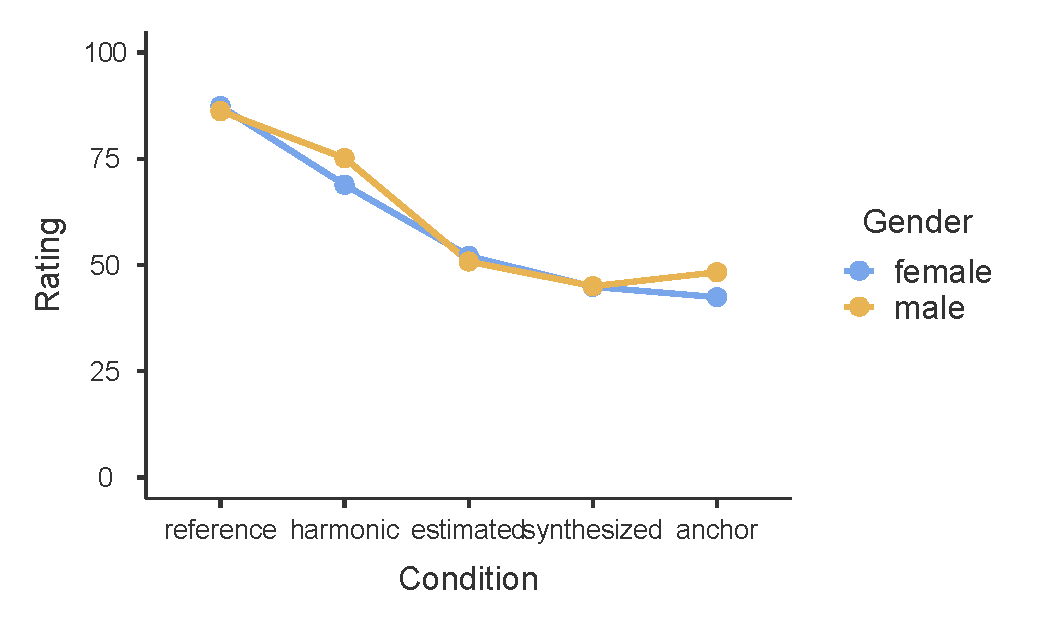
\includegraphics[width=\columnwidth]{figure_1.pdf}
\end{figure}
      
        <p></p>
      
    \begin{figure}[htbp]\caption{Vowel = i}
\label{fig:Figure_2}
% (the following arrangement follows APA7; if you want to use APA6, the caption- and label-lines have to be moved to after the includegraphics-line)
\centering
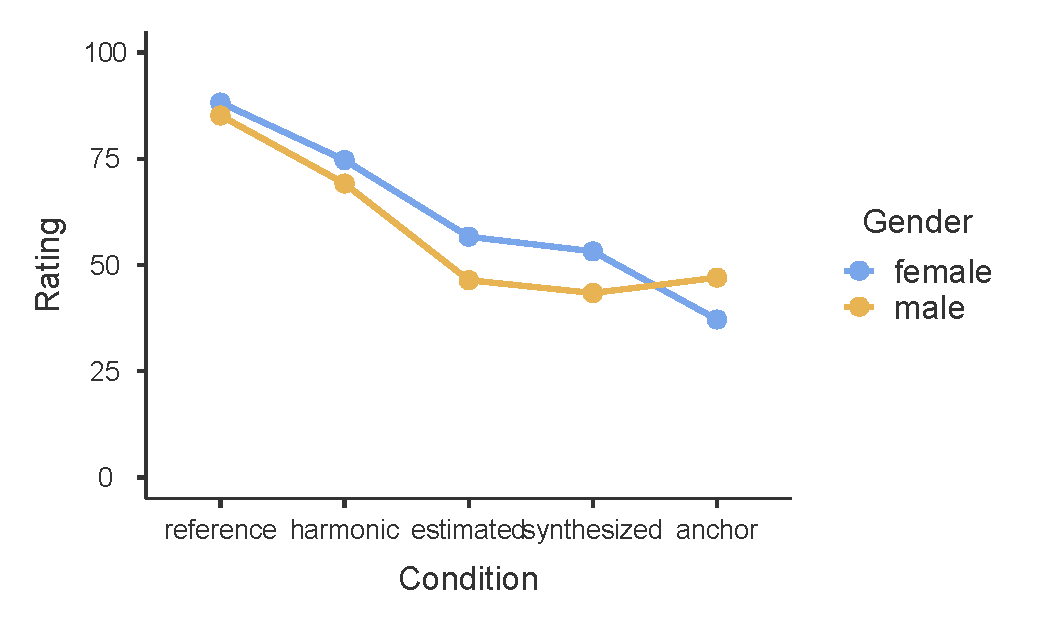
\includegraphics[width=\columnwidth]{figure_2.pdf}
\end{figure}
      
        <p></p>
      
    \begin{figure}[htbp]\caption{Vowel = o}
\label{fig:Figure_3}
% (the following arrangement follows APA7; if you want to use APA6, the caption- and label-lines have to be moved to after the includegraphics-line)
\centering
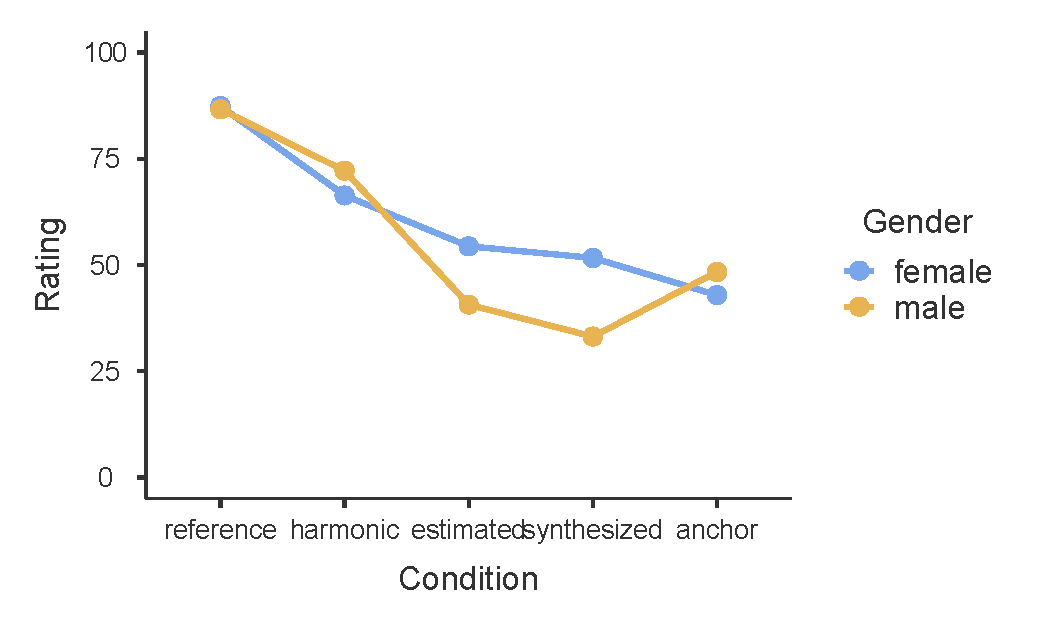
\includegraphics[width=\columnwidth]{figure_3.pdf}
\end{figure}
      
        <p></p>
      
    
      
      
    
      
        <p></p>
      
    <h2>Assumption Checks</h2>
      
        <p></p>
      
    
\begin{table}[!htbp]
\caption{Test for Normality of residuals}
\label{tab:Table_12}
\begin{adjustbox}{max size={\columnwidth}{\textheight}}
\centering
\begin{tabular}{lrr}
\hline
Test               & Statistics &               p \\
\hline
Kolmogorov-Smirnov &     0.0311 & \textless~0.001 \\
Shapiro-Wilk       &     0.9984 & \textless~0.001 \\
\hline
\end{tabular}
\end{adjustbox}
\begin{tablenotes}[para,flushleft] {
\small
}
\end{tablenotes}
\end{table}
      
        <p></p>
      
    \begin{figure}[htbp]\caption{Q-Q Plot}
\label{fig:Figure_4}
% (the following arrangement follows APA7; if you want to use APA6, the caption- and label-lines have to be moved to after the includegraphics-line)
\centering

\includegraphics[width=\columnwidth]{figure_4.pdf}
\end{figure}
      
        <p></p>
      
    \begin{figure}[htbp]\caption{Residual histogram}
\label{fig:Figure_5}
% (the following arrangement follows APA7; if you want to use APA6, the caption- and label-lines have to be moved to after the includegraphics-line)
\centering

\includegraphics[width=\columnwidth]{figure_5.pdf}
\end{figure}
      
        <p></p>
      
    
      
      
    
      
        <p></p>
      
    
      
      
    
      
        <p></p>


% =========================================================================================================

% Report your results here and make references to tables (see Table~\ref{tab:Table_1}) or figures (see Figure~\ref{fig:Figure_1}).

%\section{Discussion}
% Your discussion starts here.

%\printbibliography

%\appendix

%\section{Additional tables and figures}

%Your text introducing supplementary tables and figures.

% If required copy tables and figures from the main results here.

\end{document}

